\documentclass{IEEEtran}

\usepackage{graphicx}
\usepackage{caption}
\usepackage{subcaption}
\usepackage{hyperref}
\usepackage{url}

\bibliographystyle{plain}

\begin{document}

\title{Computational Psycholinguistics --- Assignment 2}
\author{Daan Brugmans (S1080742)}
\date{\today}

\graphicspath{{./images}}

\maketitle

\section{Introduction}
This report is the realization of the Assignment 2 project for the Radboud University course \href{https://www.ru.nl/courseguides/arts/courses/ma/rema-lc/let-rema-lcex28/}{Computational Psycholinguistics}.
For this assignment, students must investigate whether the gradients computed from a recurrent neural network correlate with measured P600 component activity from a controlled experiment.
The reasoning behind this assignment is that recent research (\cite{fitz2019erp,frank2024gradients}) has shown that the P600 component may be the backpropagation of prediction errors in the human language system.
Since neural language models also backpropagate their prediction errors using gradients, there may exist similarities between the language error backpropagation of human and artificial neural language systems.
This report contains the findings found by me for the Assignment 2 project.

The relevant code for this assignment can be found at the following URL: \url{https://github.com/daanbrugmans/ru-computational-psycholinguistics-23-24/tree/main/assignment-2/code}.

\section{Related Work}
For my realization of Assignment 2, I have chosen a controlled experiment from Kim and Osterhout (\cite{kim2005combinatory}), specifically their first experiment.
Kim and Osterhout researched P600 activity in anomalous sentences.
When they released their research, it was generally accepted that the P600 component was solely responsible for language error related to syntax, while the N400 was responsible for language error related to semantics.
In their work, Kim and Osterhout show that the P600 is still activated in sentences that are syntactically unambiguous, but have illogical semantics as a result, however.
The general structure of such sentences was one where the two agents of a sentence are swapped, maintaining a certain "theme" and a valid syntax, while going against semantics that are considered regular.
An example of this is the sentence "\textit{The hearty meal was devouring the kids}", where the syntax is unambiguous, but does imply a meaning that goes against what is usually expected of the combination of the sentence's agents and theme, which would be "\textit{The kids were devouring the hearty meal}".
The authors name such sentences \textbf{(Attraction) Violations}.

Kim and Osterhout note that Attraction Violations, especially the phrase up and including the critical verb ("\textit{The hearty meal was devouring}"), while syntactically unambiguous, can be interpreted to be either syntactically or semantically incorrect.
If a reader interprets the violation as syntactically invalid, then they likely think that the critical verb is in the wrong tense, and changing it would return the sentence to a meaning that aligns with expectations ("\textit{The hearty meal was devoured}").
If a reader interprets the violation as semantically invalid, then they likely think that the agent is wrong, and, in the case of the full sentence, that the agents should be flipped ("\textit{The kids were devouring}").
This means that an Attraction Violation can cause a syntactically unambiguous sentence to be considered syntactically invalid due to its semantics.
On the basis of this idea, Kim and Osterhout researched if sentences with Attraction Violations can trigger a P600 effect in humans.
Although P600 effects were typically taken to be responsible for purely syntactic errors at that time, syntactically unambiguous Attraction Violation sentences, which can be considered to be syntactically erroneous on the basis of the sentence's meaning, may thus elicit a P600 response based on a sentence's unexpected semantics.

\begin{figure}
    \centering
    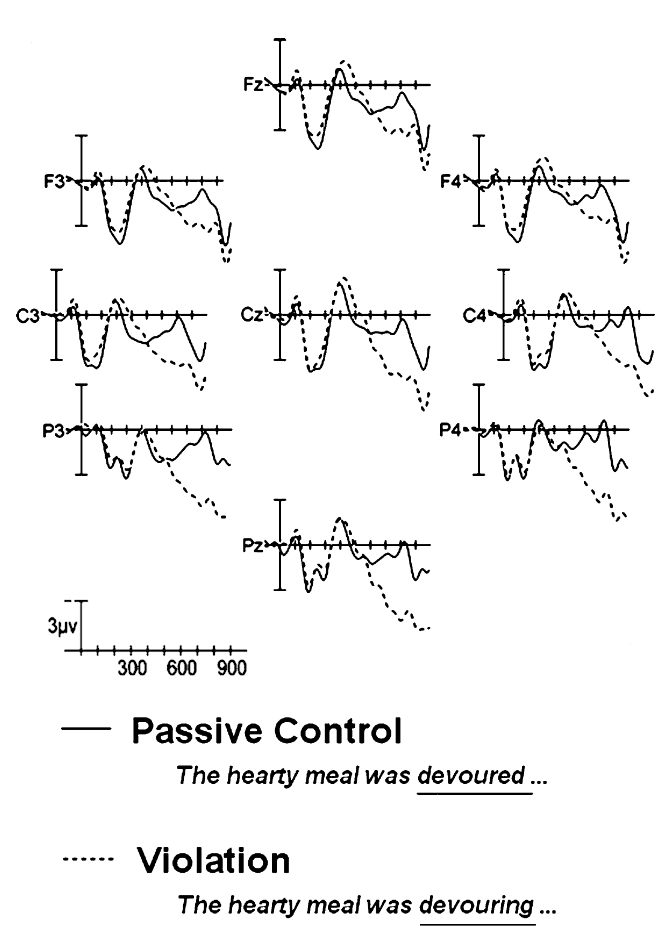
\includegraphics[width=.45\textwidth]{kim_osterhout.png}
    \caption{ERP Brain Activity when reading Violation vs. Control sentences, from \cite{kim2005combinatory}.}
    \label{fig:kim_osterhout}
\end{figure}

Kim and Osterhout conduct an experiment where participants' N400 and P600 components are read while reading both Attraction Violation sentences ("\textit{The hearty meal was devouring}"), and Control Sentences where the critical verb of the sentence is altered as to let the sentence be both syntactically and semantically coherent with its agents and theme ("\textit{The hearty meal was devoured}").
Their results show that, on the critical verb, the P600 component is much more pronounced on Attraction Violation sentences than on the Control sentences.
They also showed that the N400 component is only slightly present when Attraction Violation sentences are read, meaning that the error stemming from the sentence is mostly processed by the P600.
These findings then imply that the P600 is not responsible for syntactic error alone, and that a degree of semantic error is also processed in the P600.
A visualization of these findings can be seen in figure \ref{fig:kim_osterhout}.

\section{Methodology}
All the code I have written can be found in the Jupyter Notebook called \texttt{main.ipynb}, which should thusly contain all results also shown in this report.
It can be found at the following URL: \url{https://github.com/daanbrugmans/ru-computational-psycholinguistics-23-24/blob/main/assignment-2/code/main.ipynb}
I have placed the code in the \texttt{get\_predictions.py} file in a function called \texttt{get\_predictions}, so that I can easily call this code from the notebook.

Kim and Osterhout (\cite{kim2005combinatory}) provide their full set of Attraction Violation sentences and (Passive) Control sentences in their paper.
I have copied the full sets of these sentences up until and including the critical verb.
I have stored them as text files called \texttt{violations.txt} for the Attraction Violation sentences and \texttt{control.txt} for the Control sentences in a folder called \texttt{data}.
The notebook processes these sentences further so that they can be used by the RNNs by lowercasing all words and separating genitive markers ('s) from consonants.
Furthermore, after the surprisals and gradients have been calculated, I remove sentences that do not have surprisal and/or gradient information, and remove sentence-initial words from sentences that do.

My results are a collection of scatterplots that visualize the relationship between the surprisal and gradients of the models.
Every plot also contains a quadratic function fitted to the data to show the trend of the relationship between the variables.
I have chosen for a quadratic function as opposed to a linear function, as I found that this fits the data better.
Included in every plot is also the Pearson Correlation Coefficient \textit{r} between variables.
Since surprisal values and gradients are calculated for multiple models, I provide a plot for every model.
For every pair of variables, I also provide a plot of how the Pearson Correlation Coefficient changes as the model is trained on more data.

Before producing results, I set a universal seed for Python itself, NumPy, and PyTorch of \texttt{3131}.
I do this in order to improve the reproducibility of my results.
This is why I also set some settings for CUDA regarding PyTorch's randomness when computing on GPU.

\section{Results}
The full results can be found in the appendices, where the graphs for every model are shown for all four comparisons:
\begin{itemize}
    \item Violation Surprisal vs. Violation Gradients
    \item Control Surprisal vs. Control Gradients
    \item Violation Surprisal vs. Control Surprisal
    \item Violation Gradients vs. Control Gradients
\end{itemize}

\subsection{Comparing Surprisal vs Gradients}
\begin{figure}
    \centering
    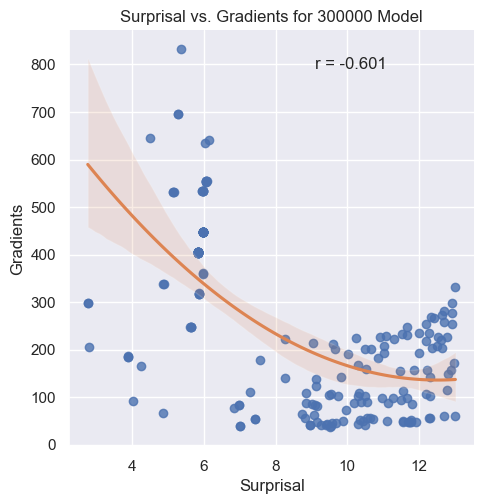
\includegraphics[width=.45\textwidth]{violations_surprisal_vs_gradients/300000.png}
    \caption{Surprisal vs. Gradients on Violations for an RNN trained on 300,000 sentences.}
    \label{fig:300000_surprisal_vs_gradients}
\end{figure}

\begin{figure*}
    \centering
    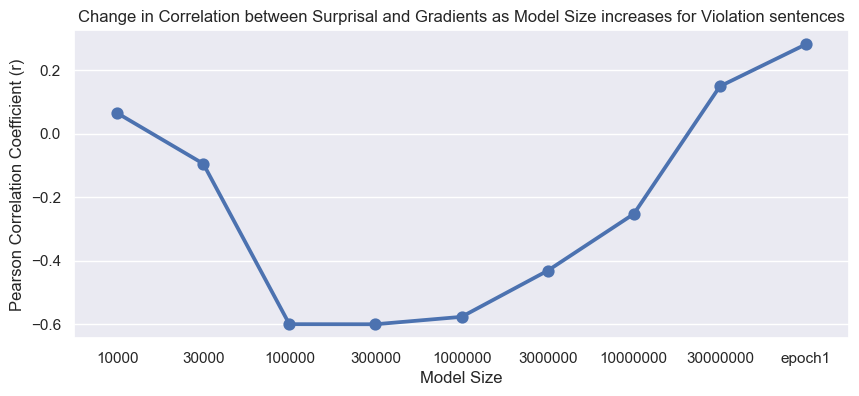
\includegraphics[width=.9\textwidth]{correlation_change/violations_surprisal_vs_gradients.png}
    \caption{The change in Correlation between Model Surprisal and Gradients on Violation Sentences as the model is trained on increasingly more data.}
    \label{fig:correlation_violations_surprisal_gradients}
\end{figure*}
\begin{figure*}
    \centering
    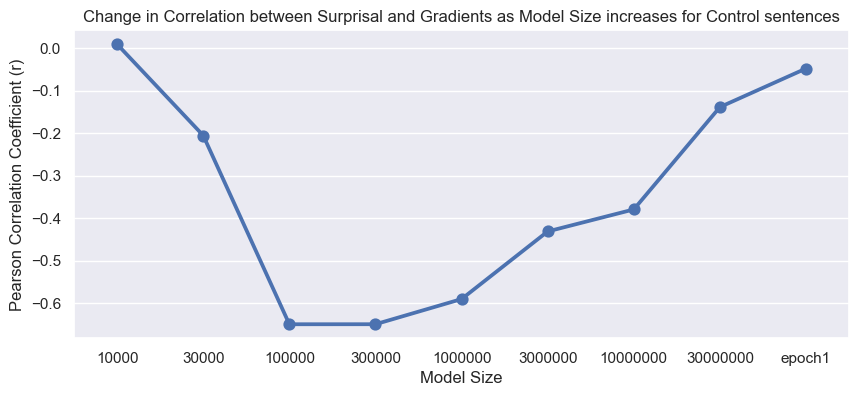
\includegraphics[width=.9\textwidth]{correlation_change/control_surprisal_vs_gradients.png}
    \caption{The change in Correlation between Model Surprisal and Gradients on Control Sentences as the model is trained on increasingly more data.}
    \label{fig:correlation_control_surprisal_gradients}
\end{figure*}

Figure \ref{fig:correlation_violations_surprisal_gradients} shows the change in Pearson Correlation Coefficient between a model's surprisal and gradients on sentences with an Attraction Violation as the model has been trained on more data.
Figure \ref{fig:correlation_control_surprisal_gradients} shows the same information, but for Control sentences.
Tables \ref{tab:correlation_violations_surprisal_gradients} and \ref{tab:correlation_control_surprisal_gradients} show the exact correlation coefficient values from these plots.
Finally, figure \ref{fig:300000_surprisal_vs_gradients} shows an example of a model's surprisals against its gradients, specifically the Recurrent Neural Network trained after 300,000 sentences.

\begin{table}
    \centering
    \begin{tabular}{c|c}
        \textbf{Trained Sentences Count} & \textbf{\textit{r}} \\
        \hline
        10,000&0.065\\
        30,000&-0.094\\
        100,000&-0.600\\
        300,000&-0.601\\
        1,000,000&-0.577\\
        3,000,000&-0.431\\
        10,000,000&-0.252\\
        30,000,000&0.149\\
        epoch1&0.282
    \end{tabular}
    \caption{Correlation Coefficients between Model Surprisal and Gradients on Violation Sentences by the model's train data size.}
    \label{tab:correlation_violations_surprisal_gradients}
\end{table}
\begin{table}
    \centering
    \begin{tabular}{c|c}
        \textbf{Trained Sentences Count} & \textbf{\textit{r}} \\
        \hline
        10,000&0.009\\
        30,000&-0.205\\
        100,000&-0.650\\
        300,000&-0.650\\
        1,000,000&-0.591\\
        3,000,000&-0.431\\
        10,000,000&-0.380\\
        30,000,000&-0.139\\
        epoch1&-0.048
    \end{tabular}
    \caption{Correlation Coefficients between Model Surprisal and Gradients on Control Sentences by the model's train data size.}
    \label{tab:correlation_control_surprisal_gradients}
\end{table}

\subsection{Comparing Conditions}
\begin{figure*}
    \centering
    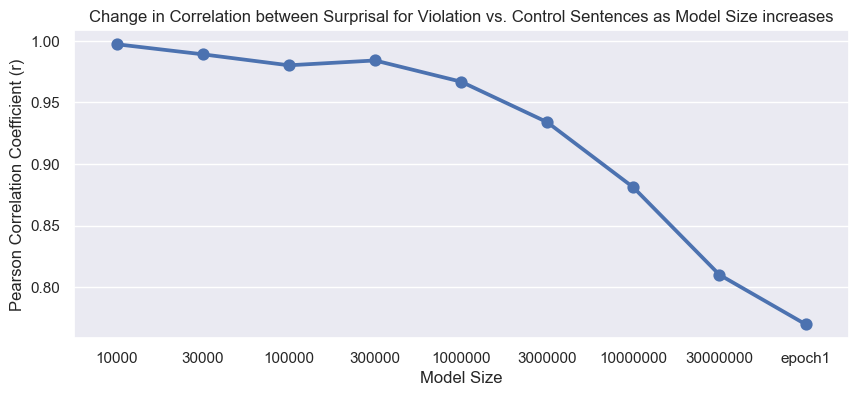
\includegraphics[width=.9\textwidth]{correlation_change/surprisal_violations_vs_control.png}
    \caption{The change in Correlation of Model Surprisal between Violation Sentences and Control Sentences as the model is trained on increasingly more data.}
    \label{fig:correlation_surprisal_violation_control}
\end{figure*}
\begin{figure*}
    \centering
    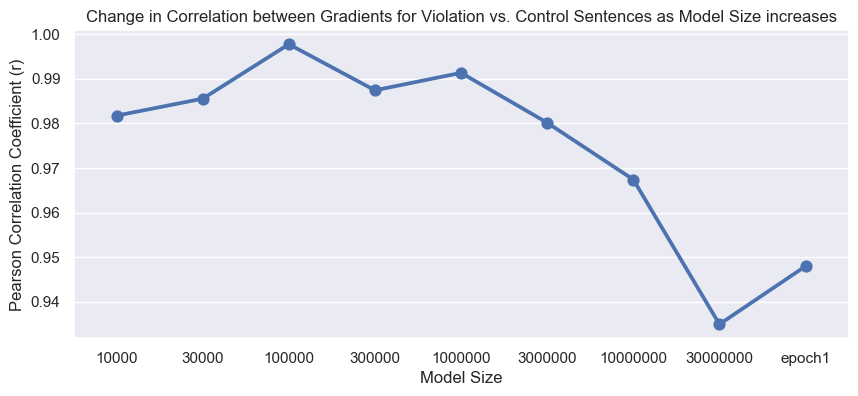
\includegraphics[width=.9\textwidth]{correlation_change/gradients_violations_vs_control.png}
    \caption{The change in Correlation of Model Gradients between Violation Sentences and Control Sentences as the model is trained on increasingly more data.}
    \label{fig:correlation_gradients_violation_control}
\end{figure*}

\begin{figure*}
    \centering
    \begin{subfigure}{0.4\textwidth}
        \centering
        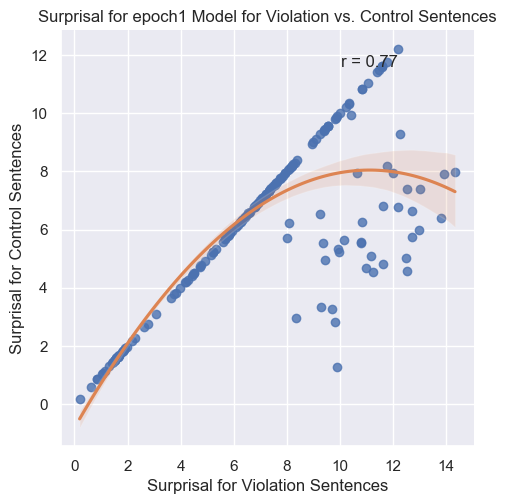
\includegraphics[width=\textwidth]{surprisal_violations_vs_control/epoch1.png}
    \end{subfigure}
    \begin{subfigure}{0.4\textwidth}
        \centering
        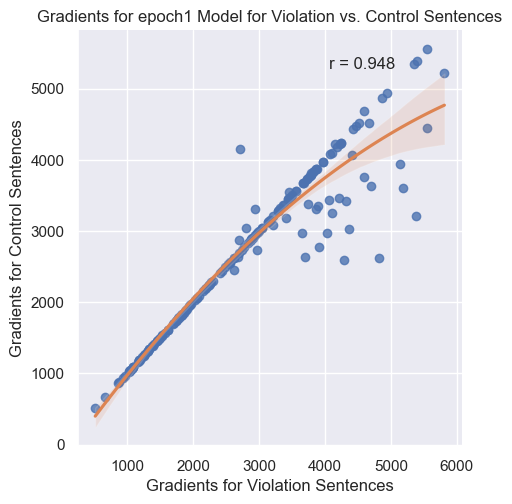
\includegraphics[width=\textwidth]{gradients_violations_vs_control/epoch1.png}
    \end{subfigure}
    \caption{Plots of the correlation between the fully trained (epoch1) model's surprisals (left) and gradients (right) on Violation Sentences vs. Control Sentences.}
    \label{fig:epoch1_correlations}
\end{figure*}

Figure \ref{fig:correlation_surprisal_violation_control} shows the change in Pearson Correlation Coefficient between a model's surprisal on sentences with an Attraction Violations versus Control sentences as the model has been trained on more data.
Figure \ref{fig:correlation_gradients_violation_control} shows the same information, but for the model's gradients.
Tables \ref{tab:correlation_surprisal_violations_control} and \ref{tab:correlation_gradients_violations_control} show the exact correlation coefficient values from these plots.
Additionally, figure \ref{fig:epoch1_correlations} shows the correlations between surprisals and gradients on the two different sentence conditions for the fully trained model.

\begin{table}
    \centering
    \begin{tabular}{c|c}
        \textbf{Trained Sentences Count} & \textbf{\textit{r}} \\
        \hline
        10,000&0.998\\
        30,000&0.990\\
        100,000&0.980\\
        300,000&0.984\\
        1,000,000&0.967\\
        3,000,000&0.934\\
        10,000,000&0.881\\
        30,000,000&0.810\\
        epoch1&0.770
    \end{tabular}
    \caption{Correlation Coefficients between Model Surprisals of Violation Sentences and Control Sentences by the model's train data size.}
    \label{tab:correlation_surprisal_violations_control}
\end{table}
\begin{table}
    \centering
    \begin{tabular}{c|c}
        \textbf{Trained Sentences Count} & \textbf{\textit{r}} \\
        \hline
        10,000&0.981\\
        30,000&0.986\\
        100,000&0.998\\
        300,000&0.987\\
        1,000,000&0.991\\
        3,000,000&0.980\\
        10,000,000&0.967\\
        30,000,000&0.935\\
        epoch1&0.947
    \end{tabular}
    \caption{Correlation Coefficients between Model Gradients of Violation Sentences and Control Sentences by the model's train data size.}
    \label{tab:correlation_gradients_violations_control}
\end{table}

\section{Discussion}
\subsection{Correlations between Surprisal and Gradients}
The data in figures \ref{fig:correlation_violations_surprisal_gradients} and \ref{fig:correlation_control_surprisal_gradients} show an interesting trend in the predictive power of a model's surprisal for its gradients: the strength of the correlation between the variables gets stronger as the model has trained on more data.
This strength reaches a peak of -0.6 to -0.65 when the model is trained on 300,000 sentences, after which, the correlation strength starts to move into the opposite direction; it returns to zero and grows from negative to positive.
I expect that the increasing strength of the correlation until 300,000 sentences can be explained by the learning process of the model.
As the model has learned more, its gradients become a better representation of its surprisal, because it has gained an understanding of the data it has learned.
When it has reached this depth of understanding, words that it expects backpropagate with small losses, while words that it is surprised by backpropagate with large losses.
As the model continues to learn, the surprisal starts to become a worse predictor of the gradients.
I expect this is due to overfitting: the model doesn't learn from being surprised by words anymore, so the backpropagated losses represent other information that it is learning.
Since these losses represent more than just surprisal, they become less correlated with surprisal.
Based on this explanation, we will assume that the model's gradients are best explained by its surprisals and vice versa for the model trained on 300,00 sentences.
Figure \ref{fig:300000_surprisal_vs_gradients} shows the exact way in which the relationship between surprisals and gradients develops for the model trained on 300,00 sentences: higher surprisals are more common than lower surprisals, and as the size of the surprisal increases, the size of the gradients tends to decrease.

\subsection{Correlations between Conditions}
Figures \ref{fig:correlation_surprisal_violation_control} and \ref{fig:correlation_gradients_violation_control} show the change between sentence conditions (Violation vs. Control) for a model's surprisal/gradients as the model is trained on more sentence data.
These correlations stand for how similar the surprisals and gradients are between conditions: the higher the correlation, the more similar they are.
A lower correlation between conditions then implies a greater difference in surprisal/gradients between the critical verbs of Violation sentences vs. Control sentences.
This disparity between conditions says something about the effect strength of the anomalies in the Violation sentences: lower correlations imply that the syntactic/semantic anomalies have a bigger effect on the model's surprisal/gradients.

The trend in figure \ref{fig:correlation_surprisal_violation_control} is clear: as the model has trained on more sentence data, the correlation decreases, and does so at an accelerating rate.
This would imply that, as the model is trained on more data, it should be more surprised about the critical verbs in Violation sentences.
The left plot of figure \ref{fig:epoch1_correlations} shows this in practice: the diagonal line in the plot is the collection of words preceding the critical verb, while the points off this line are the critical verbs.
It can be seen that these critical verbs have higher surprisals in the Violation sentences than in the Control sentences.
Thus, as a model has learned on more data, it becomes more surprised at unexpected words.

The trend of decreasing correlations across conditions does not seem to hold to the same degree for gradients, however.
Figure \ref{fig:correlation_gradients_violation_control} shows that there exists only a slight decrease in correlation as the model is trained on more sentence data.
The right plot of figure \ref{fig:epoch1_correlations} shows the details: the diagonal line stands for words preceding the critical verb, while the points off this line are the critical verbs.
It can be seen that the critical verbs tend to elicit a greater backpropagation gradient in Violation sentences than Control sentences, although this is not always the case.

\subsection{Correlations with ERP Components}
We have seen that, in our results, the anomalous critical verbs in Attraction Violation sentences have a bigger effect on the model's surprisal than on the model's gradients.
If we follow the work by Frank (\cite{frank2024gradients}) and assume that model surprisal correlates with the N400, and that model gradients correlate with the P600, then the greater disparity between sentence conditions for model surprisal than model gradients would have us expect that in Attraction Violation sentences, the N400 would be more active than the P600.
However, this goes against the findings by Kim and Osterhout (\cite{kim2005combinatory}), who show that the P600 is much more active when reading Violation sentences than the N400.
I expect that this contrast may have something to do with how the model perceives the critical verb: as either a syntactic anomaly, or a semantic anomaly.
Since the N400 is thought to represent semantic language-error, and since it correlates with model surprisal, it could be possible that the model's surprisal is more effected by the critical verbs than its gradients because it considers the Violation sentence to be semantically anomalous, and not syntactically anomalous.
It may be that the model, at the critical verb, recognizes that the semantics of the sentence do not make sense given the current syntax, which acknowledges the problem that this syntactically unambiguous sentence may need a syntactic change in order to become semantically expected, which is also a problem acknowledged in the work by Kim and Osterhout.

\section{Conclusions}
From my findings, I would not conclude that the P600 component can be explained by model surprisal or gradients, since they seem to go against earlier findings by Kim and Osterhout (\cite{kim2005combinatory}) and Frank (\cite{frank2024gradients}).
However, it is clear that model surprisal and its gradients are effected by anomalous critical verbs, so there certainly is a component of language-error processing being performed by the model on the anomalous critical verbs, akin to the theorized backpropagation of language error by the P600.
So, although I would not conclude that the P600 can be explained by either the model's surprisals or gradients, I would conclude that the unexpectedness of a word influences the size of the backpropagated gradients.

\bibliography{bib}

\onecolumn
\appendix
% \section*{Appendix A: Plots of Model Surprisal vs. Model Gradients}
% \begin{figure*}[h]
%     \centering
%     \begin{subfigure}{0.4\textwidth}
%         \centering
%         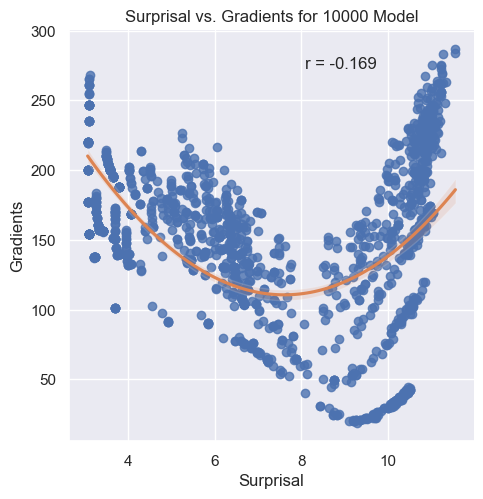
\includegraphics[width=\textwidth]{surprisal_vs_gradients/10000.png}
%     \end{subfigure}
%     \begin{subfigure}{0.4\textwidth}
%         \centering
%         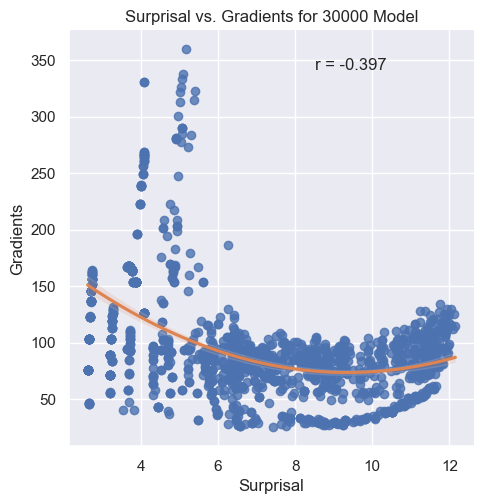
\includegraphics[width=\textwidth]{surprisal_vs_gradients/30000.png}
%     \end{subfigure}
% \end{figure*}
% \begin{figure*}[h]
% \centering
% \begin{subfigure}{0.4\textwidth}
%     \centering
%     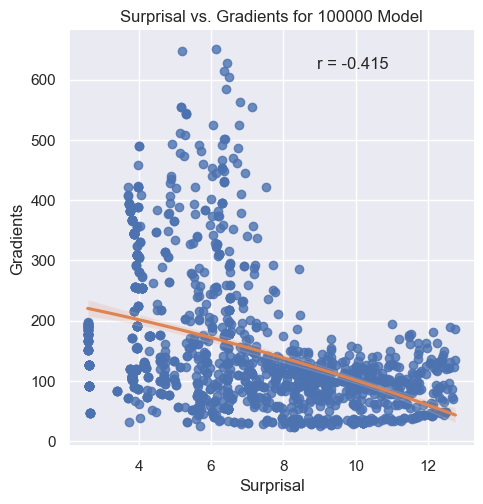
\includegraphics[width=\textwidth]{surprisal_vs_gradients/100000.png}
% \end{subfigure}
% \begin{subfigure}{0.4\textwidth}
%     \centering
%     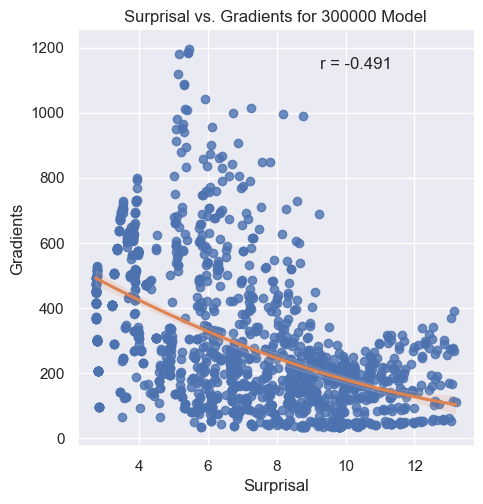
\includegraphics[width=\textwidth]{surprisal_vs_gradients/300000.png}
% \end{subfigure}
% \end{figure*}
% \begin{figure*}[h]
%     \centering
%     \begin{subfigure}{0.4\textwidth}
%         \centering
%         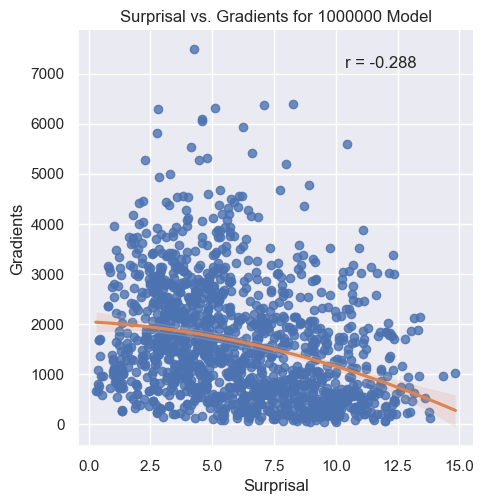
\includegraphics[width=\textwidth]{surprisal_vs_gradients/1000000.png}
%     \end{subfigure}
%     \begin{subfigure}{0.4\textwidth}
%         \centering
%         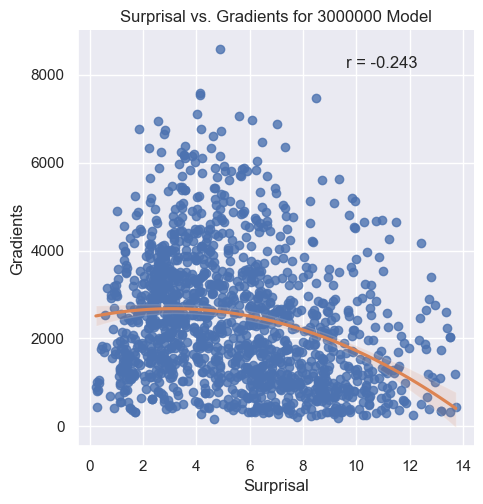
\includegraphics[width=\textwidth]{surprisal_vs_gradients/3000000.png}
%     \end{subfigure}
% \end{figure*}
% \begin{figure*}[h]
%     \centering
%     \begin{subfigure}{0.4\textwidth}
%         \centering
%         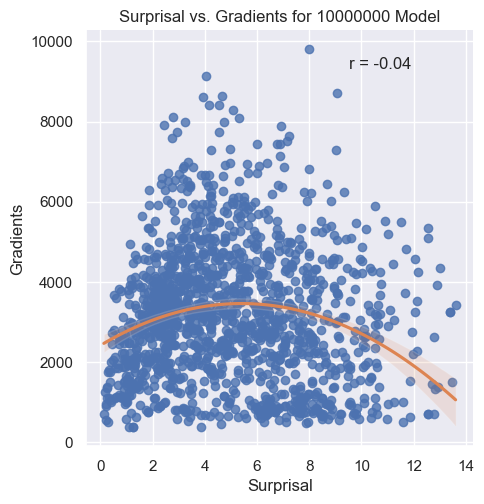
\includegraphics[width=\textwidth]{surprisal_vs_gradients/10000000.png}
%     \end{subfigure}
%     \begin{subfigure}{0.4\textwidth}
%         \centering
%         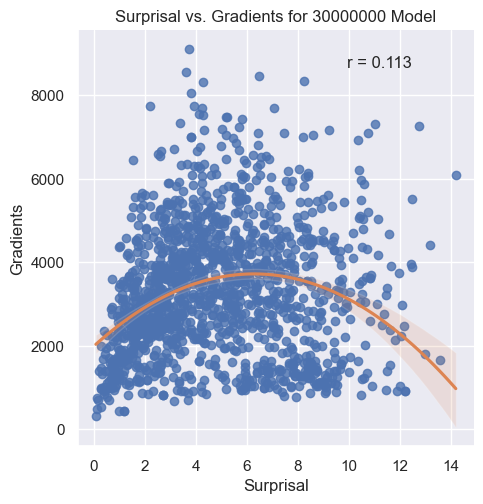
\includegraphics[width=\textwidth]{surprisal_vs_gradients/30000000.png}
%     \end{subfigure}
% \end{figure*}
% \begin{figure*}[h]
%     \centering
%     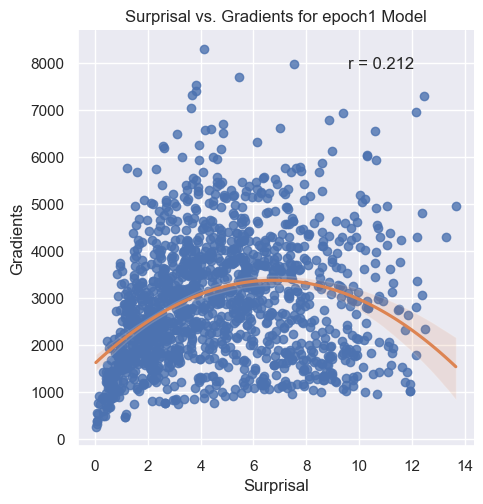
\includegraphics[width=0.4\textwidth]{surprisal_vs_gradients/epoch1.png}
% \end{figure*}

% \clearpage

% \section*{Appendix B: Plots of Model Gradients vs. Mean P600 Component}
% \begin{figure*}[h]
%     \centering
%     \begin{subfigure}{0.4\textwidth}
%         \centering
%         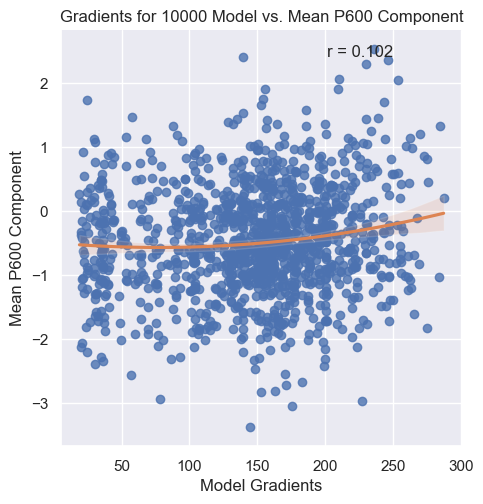
\includegraphics[width=\textwidth]{gradients_vs_p600/10000.png}
%     \end{subfigure}
%     \begin{subfigure}{0.4\textwidth}
%         \centering
%         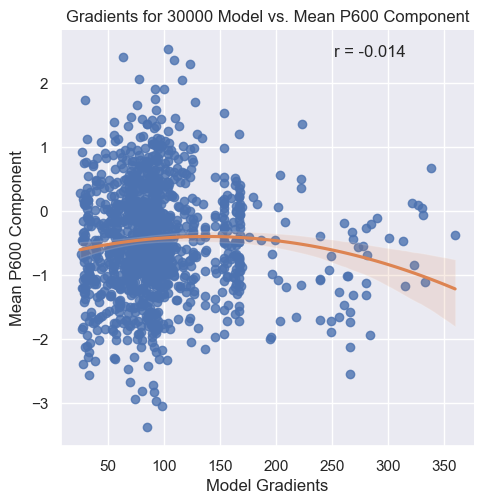
\includegraphics[width=\textwidth]{gradients_vs_p600/30000.png}
%     \end{subfigure}
% \end{figure*}
% \begin{figure*}[h]
% \centering
% \begin{subfigure}{0.4\textwidth}
%     \centering
%     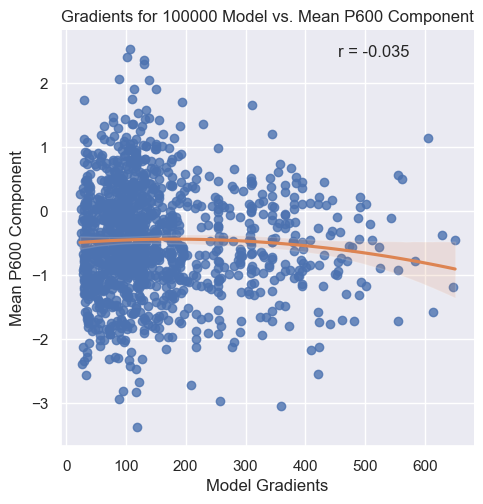
\includegraphics[width=\textwidth]{gradients_vs_p600/100000.png}
% \end{subfigure}
% \begin{subfigure}{0.4\textwidth}
%     \centering
%     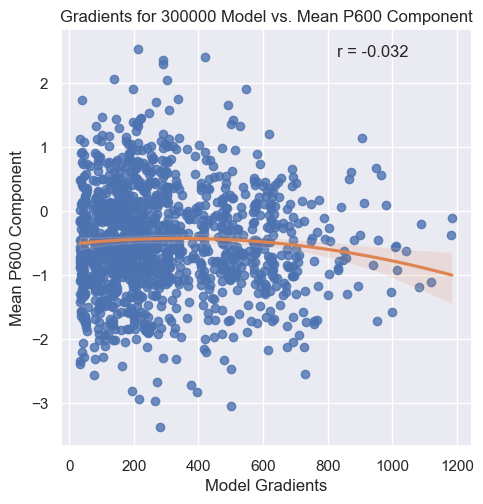
\includegraphics[width=\textwidth]{gradients_vs_p600/300000.png}
% \end{subfigure}
% \end{figure*}
% \begin{figure*}[h]
%     \centering
%     \begin{subfigure}{0.4\textwidth}
%         \centering
%         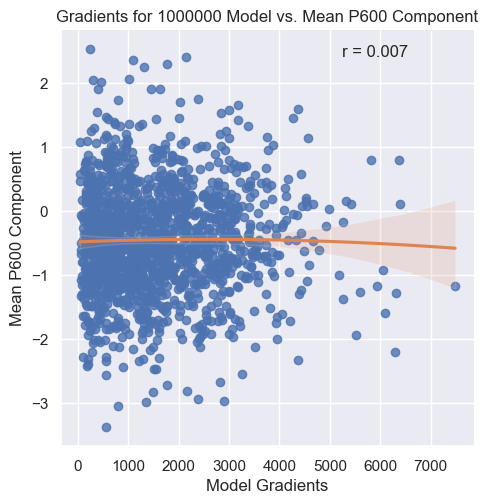
\includegraphics[width=\textwidth]{gradients_vs_p600/1000000.png}
%     \end{subfigure}
%     \begin{subfigure}{0.4\textwidth}
%         \centering
%         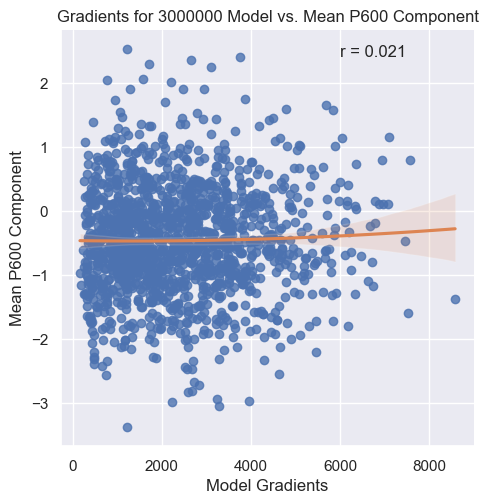
\includegraphics[width=\textwidth]{gradients_vs_p600/3000000.png}
%     \end{subfigure}
% \end{figure*}
% \begin{figure*}[h]
%     \centering
%     \begin{subfigure}{0.4\textwidth}
%         \centering
%         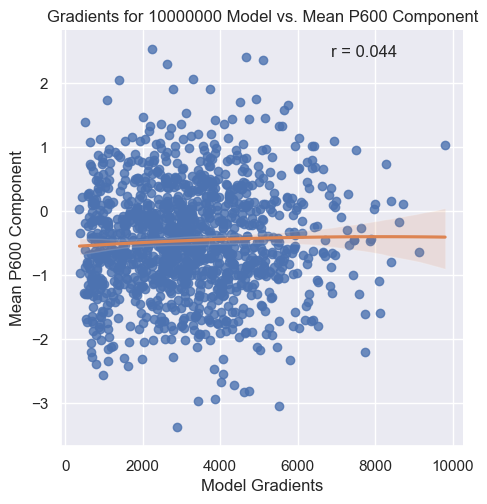
\includegraphics[width=\textwidth]{gradients_vs_p600/10000000.png}
%     \end{subfigure}
%     \begin{subfigure}{0.4\textwidth}
%         \centering
%         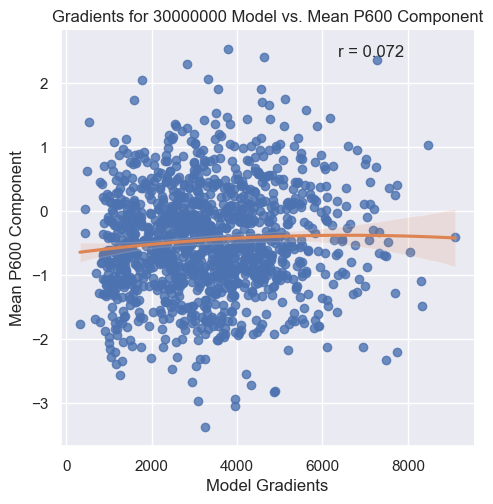
\includegraphics[width=\textwidth]{gradients_vs_p600/30000000.png}
%     \end{subfigure}
% \end{figure*}
% \begin{figure*}[h]
%     \centering
%     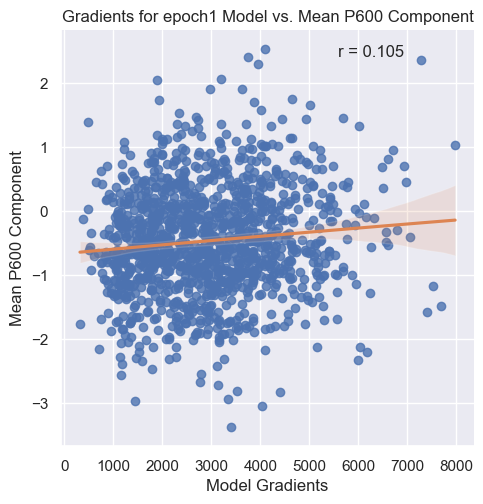
\includegraphics[width=0.4\textwidth]{gradients_vs_p600/epoch1.png}
% \end{figure*}

% \clearpage

% \section*{Appendix C: Plots of Model Surprisal vs. Mean P600 Component}
% \begin{figure*}[h]
%     \centering
%     \begin{subfigure}{0.4\textwidth}
%         \centering
%         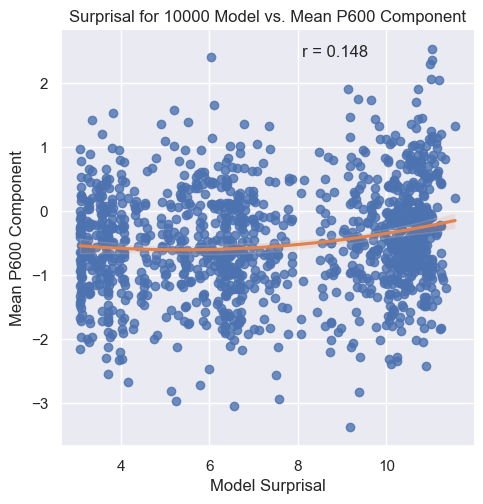
\includegraphics[width=\textwidth]{surprisal_vs_p600/10000.png}
%     \end{subfigure}
%     \begin{subfigure}{0.4\textwidth}
%         \centering
%         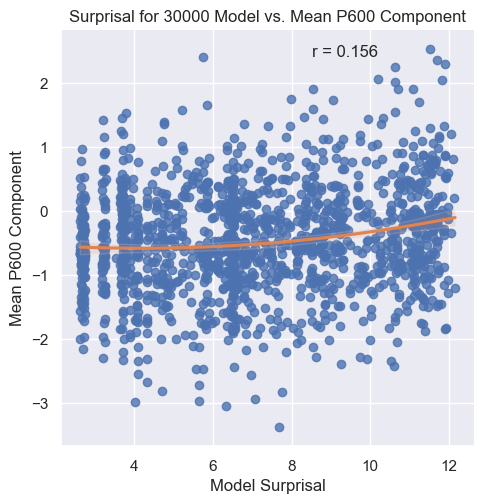
\includegraphics[width=\textwidth]{surprisal_vs_p600/30000.png}
%     \end{subfigure}
% \end{figure*}
% \begin{figure*}[h]
% \centering
% \begin{subfigure}{0.4\textwidth}
%     \centering
%     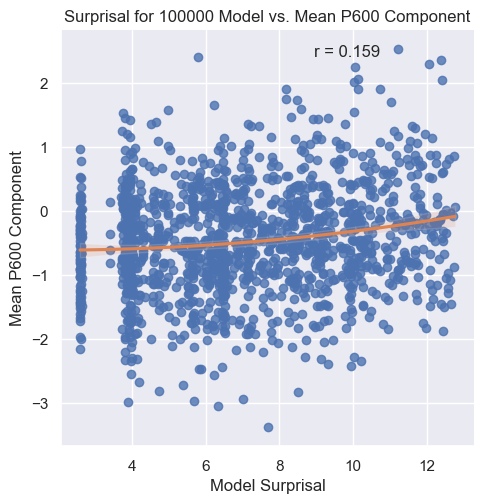
\includegraphics[width=\textwidth]{surprisal_vs_p600/100000.png}
% \end{subfigure}
% \begin{subfigure}{0.4\textwidth}
%     \centering
%     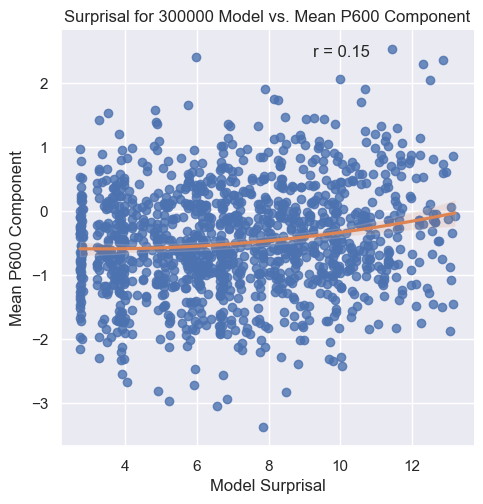
\includegraphics[width=\textwidth]{surprisal_vs_p600/300000.png}
% \end{subfigure}
% \end{figure*}
% \begin{figure*}[h]
%     \centering
%     \begin{subfigure}{0.4\textwidth}
%         \centering
%         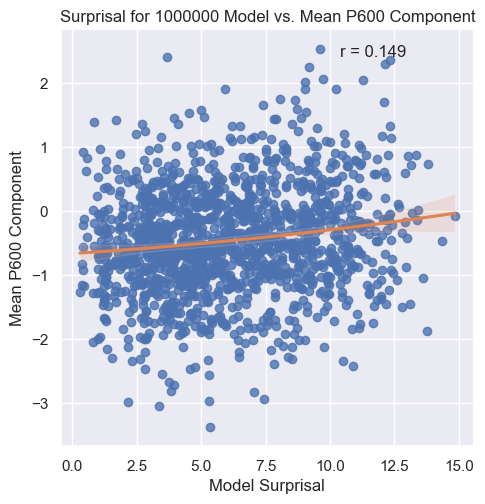
\includegraphics[width=\textwidth]{surprisal_vs_p600/1000000.png}
%     \end{subfigure}
%     \begin{subfigure}{0.4\textwidth}
%         \centering
%         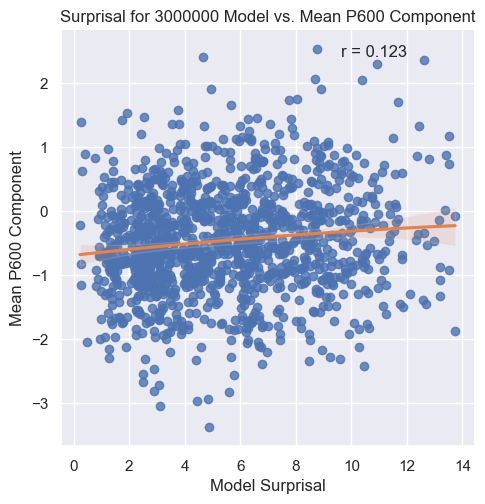
\includegraphics[width=\textwidth]{surprisal_vs_p600/3000000.png}
%     \end{subfigure}
% \end{figure*}
% \begin{figure*}[h]
%     \centering
%     \begin{subfigure}{0.4\textwidth}
%         \centering
%         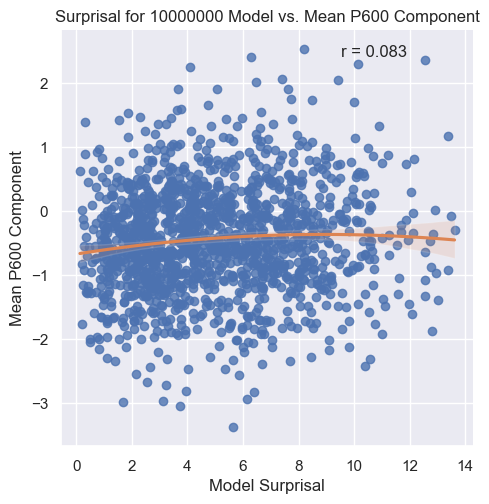
\includegraphics[width=\textwidth]{surprisal_vs_p600/10000000.png}
%     \end{subfigure}
%     \begin{subfigure}{0.4\textwidth}
%         \centering
%         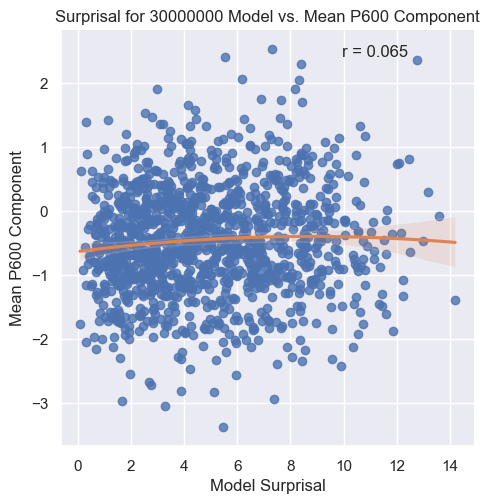
\includegraphics[width=\textwidth]{surprisal_vs_p600/30000000.png}
%     \end{subfigure}
% \end{figure*}
% \begin{figure*}[h]
%     \centering
%     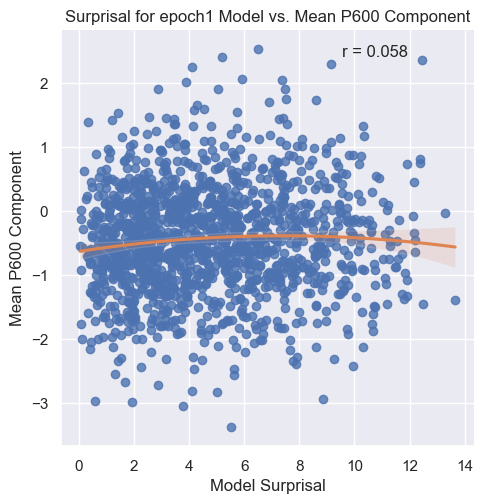
\includegraphics[width=0.4\textwidth]{surprisal_vs_p600/epoch1.png}
% \end{figure*}

\end{document}